\documentclass[hyperref={pdfpagelabels=false}]{beamer}

%\usepackage{lmodern}
\usepackage{graphicx}
\usepackage{epstopdf}
\usepackage{natbib}
\usepackage{adforn}
\usepackage{multimedia}

\usefonttheme{professionalfonts} % using non standard fonts for beamer
\usefonttheme{serif} % default family is serif
\usepackage[T1]{fontenc}
\usepackage{newtxtext,newtxmath}
\usepackage{verbatim}

\input{../TeX/supplement/customizations}

\bibpunct[:]{(}{)}{;}{a}{}{,}
\bibliographystyle{yahapj}

\usepackage{aastex_hack}
\usepackage{tikz}

%\usetheme{Madrid}
\usetheme{CambridgeUS}
\usecolortheme{seagull}
\setbeamertemplate{itemize items}{\adforn{3}}
\setbeamertemplate{enumerate items}[default]
\setbeamertemplate{title page}[default][colsep=-4bp,rounded=true]
\setbeamertemplate{frametitle}[default][center]

\title[{\normalfont\scshape Optical Variability Signatures from Massive Black Hole Binaries}]{{\normalfont\scshape Optical Variability Signatures from Massive Black Hole Binaries}}
\subtitle{{\tiny 229$^{\mathrm{th}}$ American Astronomical Society Meeting Grapevine, TX}}
\author[{\normalfont\scshape Vishal Pramod Kasliwal}]{{\normalfont\scshape Vishal Pramod Kasliwal} \\ {\tiny {\texttt{vishal.kasliwal@gmail.com}}}}
\institute[]
{
  Department of Physics \& Astronomy \\
  University of Pennsylvania \\
  \& \\
  Dept. of Astrophysical Sciences \\
  Princeton University
}
\date{January 07$^{\mathrm{th}}$, 2017}
\begin{document}

\begin{frame}
\titlepage
\end{frame}

\normalfont\normalfont

\section{Massive Black Hole Binaries}

\subsection{Introduction}

\begin{frame}
\frametitle{Galaxy Mergers $\implies$ Massive Black Hole Binaries (MBHB)}
  \begin{figure}
    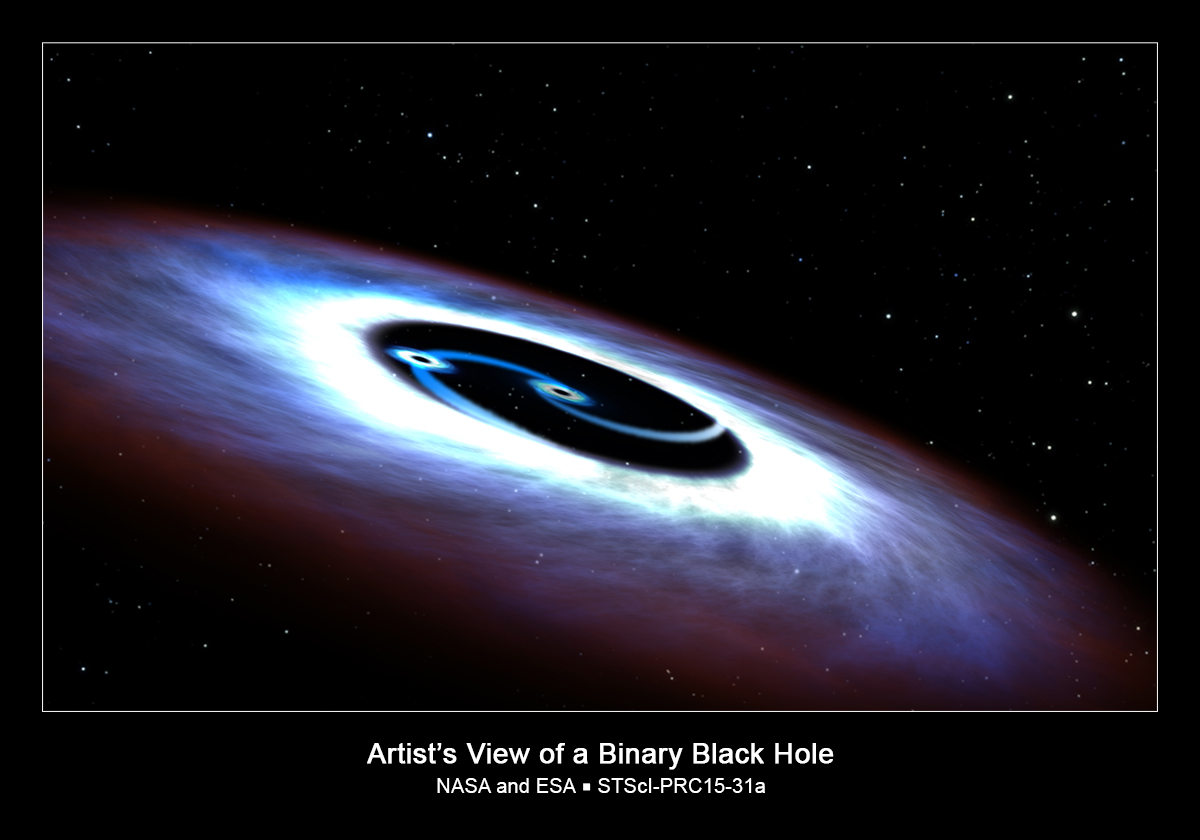
\includegraphics[scale=0.75]{images/BinaryBlackHole.jpg}
  \end{figure}
  \begin{columns}
    \centering
    \begin{column}{0.35\textwidth}
      \begin{itemize}
        \item {\scriptsize \citet{ShenLoeb10}}
        \item {\scriptsize \citet{ColpiAccretion}}
      \end{itemize}
    \end{column}
    \begin{column}{0.35\textwidth}
      \begin{itemize}
        \item {\scriptsize \citet{DOrazio13}}
        \item {\scriptsize \citet{binarySMBHNature15}}
      \end{itemize}
    \end{column}
\end{columns}
\end{frame}

\begin{frame}
\frametitle{AGN Show Complex Variability Behavior}
  \begin{columns}
    \centering
    \begin{column}{0.35\textwidth}
      \begin{figure}
        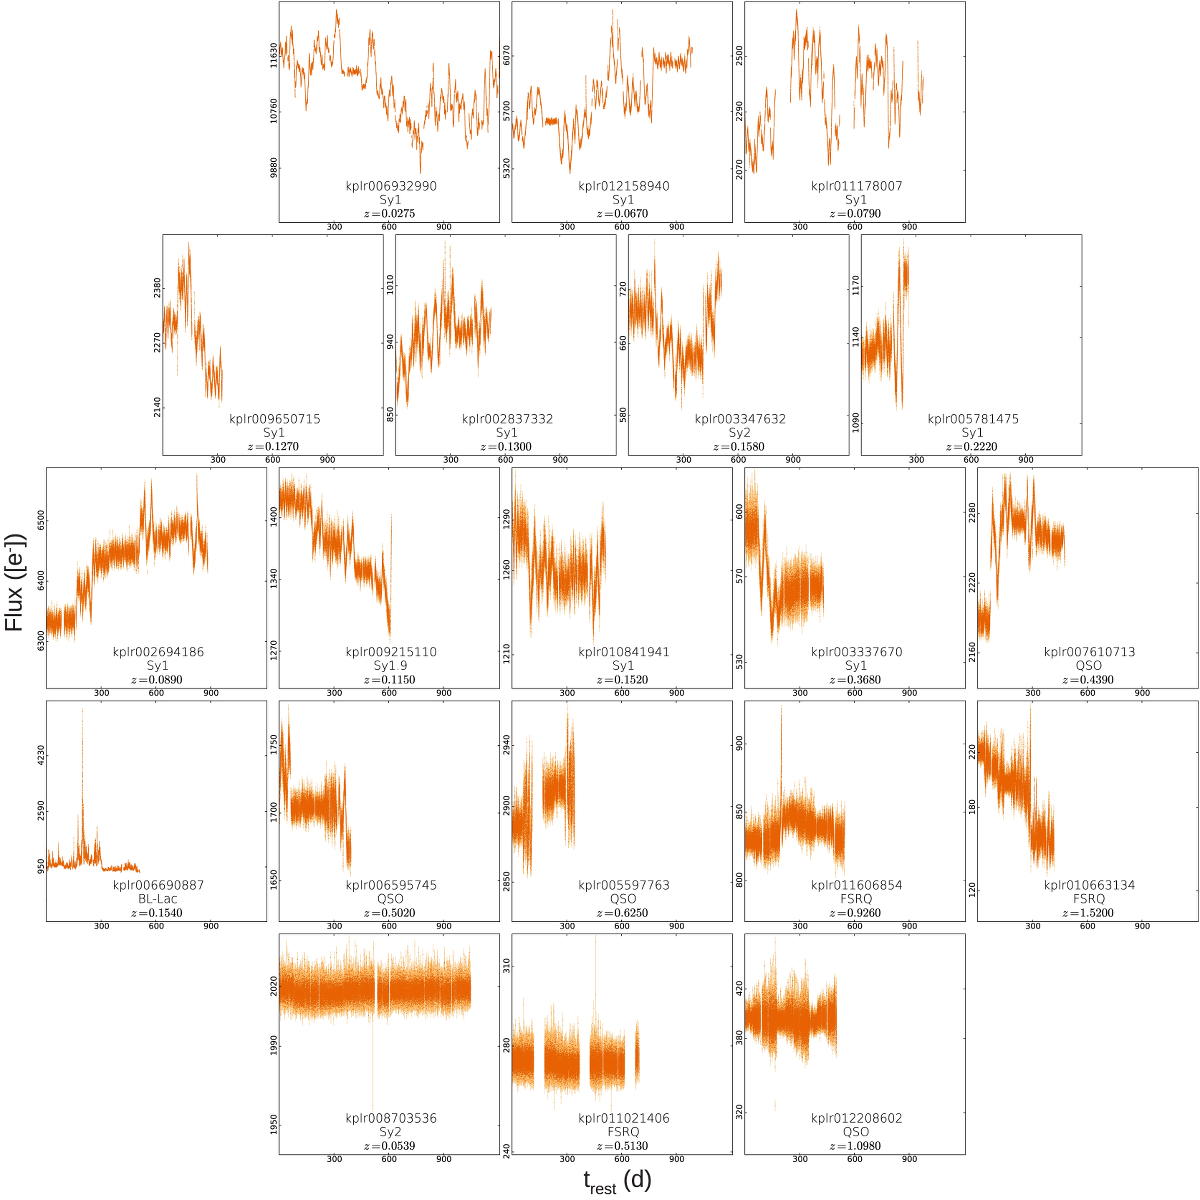
\includegraphics[scale=0.32]{images/AllLC.jpg}
      \end{figure}
    \end{column}
    \begin{column}{0.35\textwidth}
        \begin{figure}
          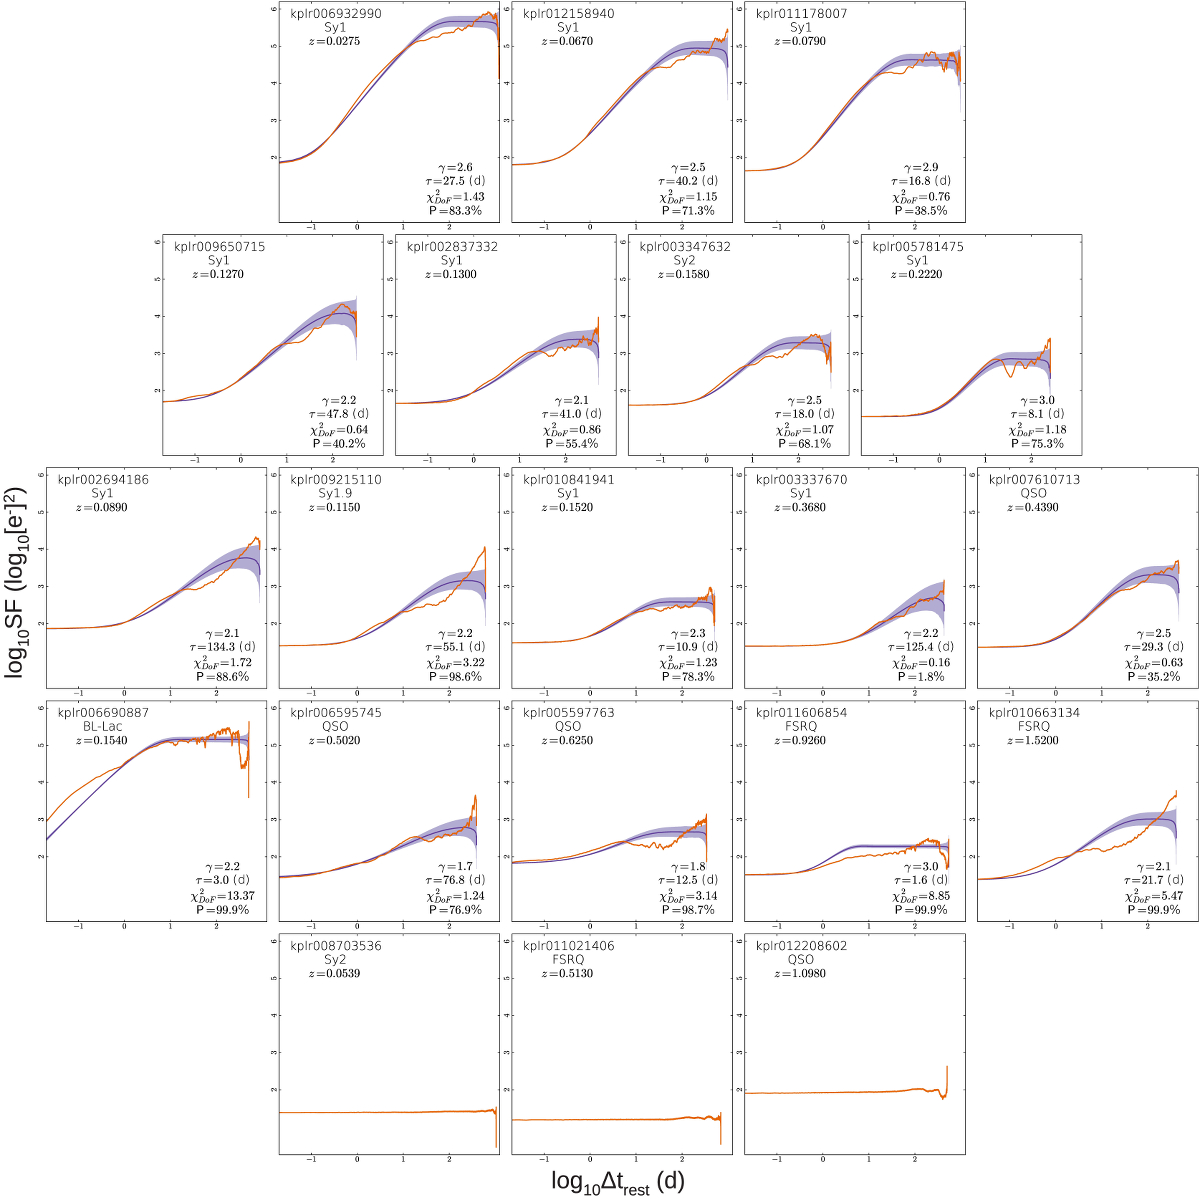
\includegraphics[scale=0.32]{images/AllSF.jpg}
        \end{figure}
    \end{column}
  \end{columns}
  \begin{columns}
    \centering
    \begin{column}{0.35\textwidth}
      \begin{itemize}
        \item {\footnotesize $z \sim 0.02$-$1.5$}
        \item {\footnotesize $\delta t_{\mathrm{rest}} \sim 14$-$28$~min}
        \item {\footnotesize $N \sim 16$k-$60$k}
        %\item Wide variety of behavior!
      \end{itemize}
    \end{column}
    \begin{column}{0.35\textwidth}
      \begin{itemize}
        \item {\footnotesize PSD index $-1.7 \sim -3.1$}
        %\item Not all AGN $\sim$ DRW
        \item {\footnotesize PSD model too simple}
        \item {\footnotesize Onset over $\sim 1$~hr to $\sim 1$~d}
      \end{itemize}
    \end{column}
  \end{columns}
\end{frame}

\section{Modelling AGN Variability as a C-ARMA Process}

\subsection{What is a C-ARMA Process?}

\begin{frame}
\frametitle{Continuous-time AutoRegressive Moving Average (C-ARMA) Processes}
  \begin{equation*} \mathrm{d}W \sim \mathcal{N}(0,\mathrm{d}t) \end{equation*}
  \begin{equation*}\label{eq:CARMA} \mathrm{d}^{p}x + \alpha_{1} \mathrm{d}^{p-1}x + \ldots + \alpha_{p-1} \mathrm{d}x + \alpha_{p}x = \beta_{0} (\mathrm{d}W) + \ldots + \beta_{q} \mathrm{d}^{q}(\mathrm{d}W) \end{equation*}
  \begin{columns}
    \centering
    \begin{column}{0.5\textwidth}
      \begin{itemize}
        {\scriptsize \item It\={o} calculus {\tiny \citet{Davis,Brockwell14,Kelly14,KasliwalCARMA}}}
        {\scriptsize \item Drive linearized system with noise}
        {\scriptsize \item PSD is a ratio of even polynomials in frequency}
        \item Modulate C-ARMA with relativistic beaming factor!
        \item Now available in \href{https://github.com/AstroVPK/kali}{\textsc{k\={a}l\={i}}}!
      \end{itemize}
    \end{column}
    \begin{column}{0.5\textwidth}
      \begin{figure}
        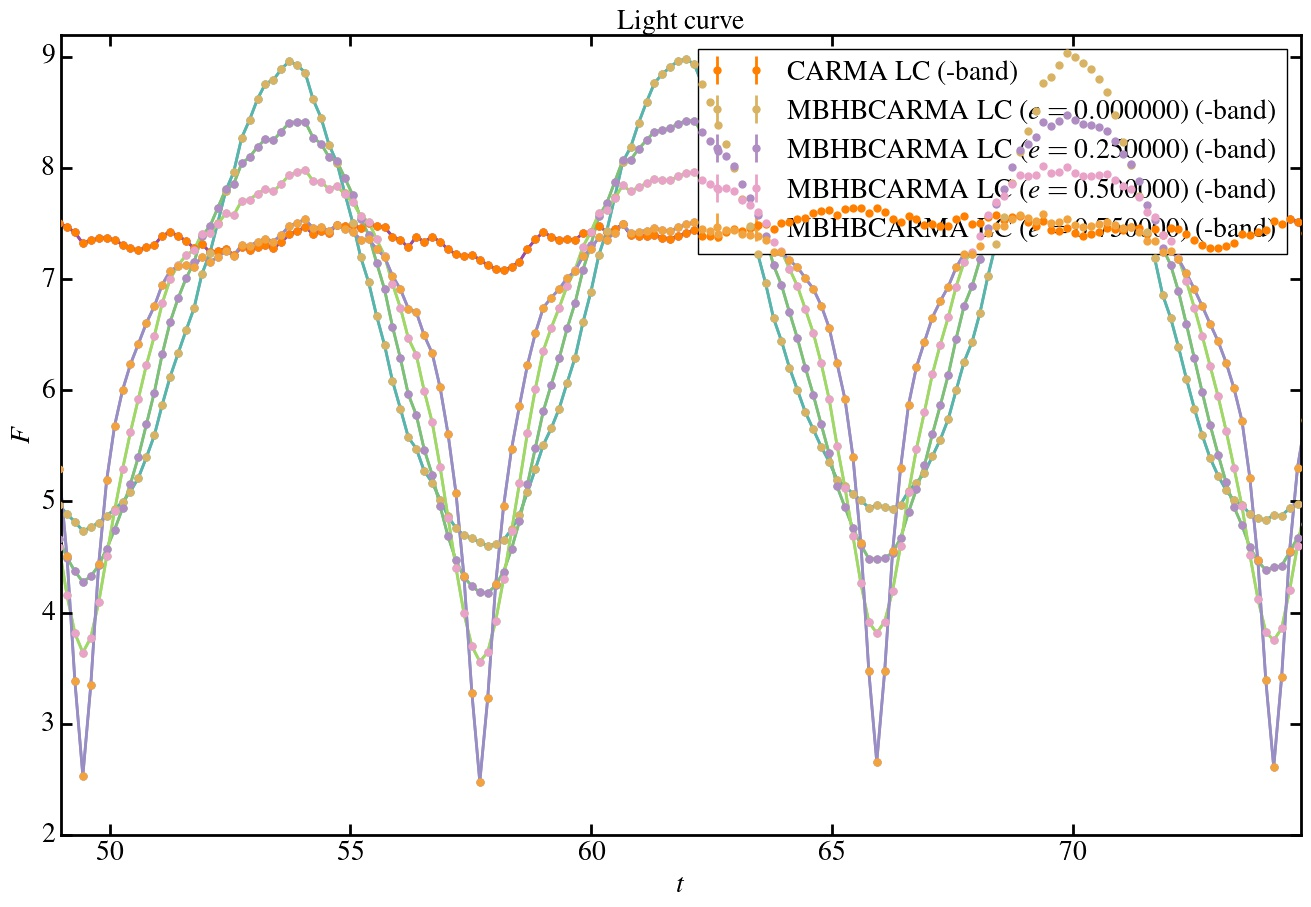
\includegraphics[scale=0.125]{images/MBHBLCs.jpg}
      \end{figure}
    \end{column}
  \end{columns}
\end{frame}

\begin{frame}
\frametitle{Effect on PSD}
  \begin{columns}
  \centering
    \begin{column}{0.5\textwidth}
      \begin{figure}
        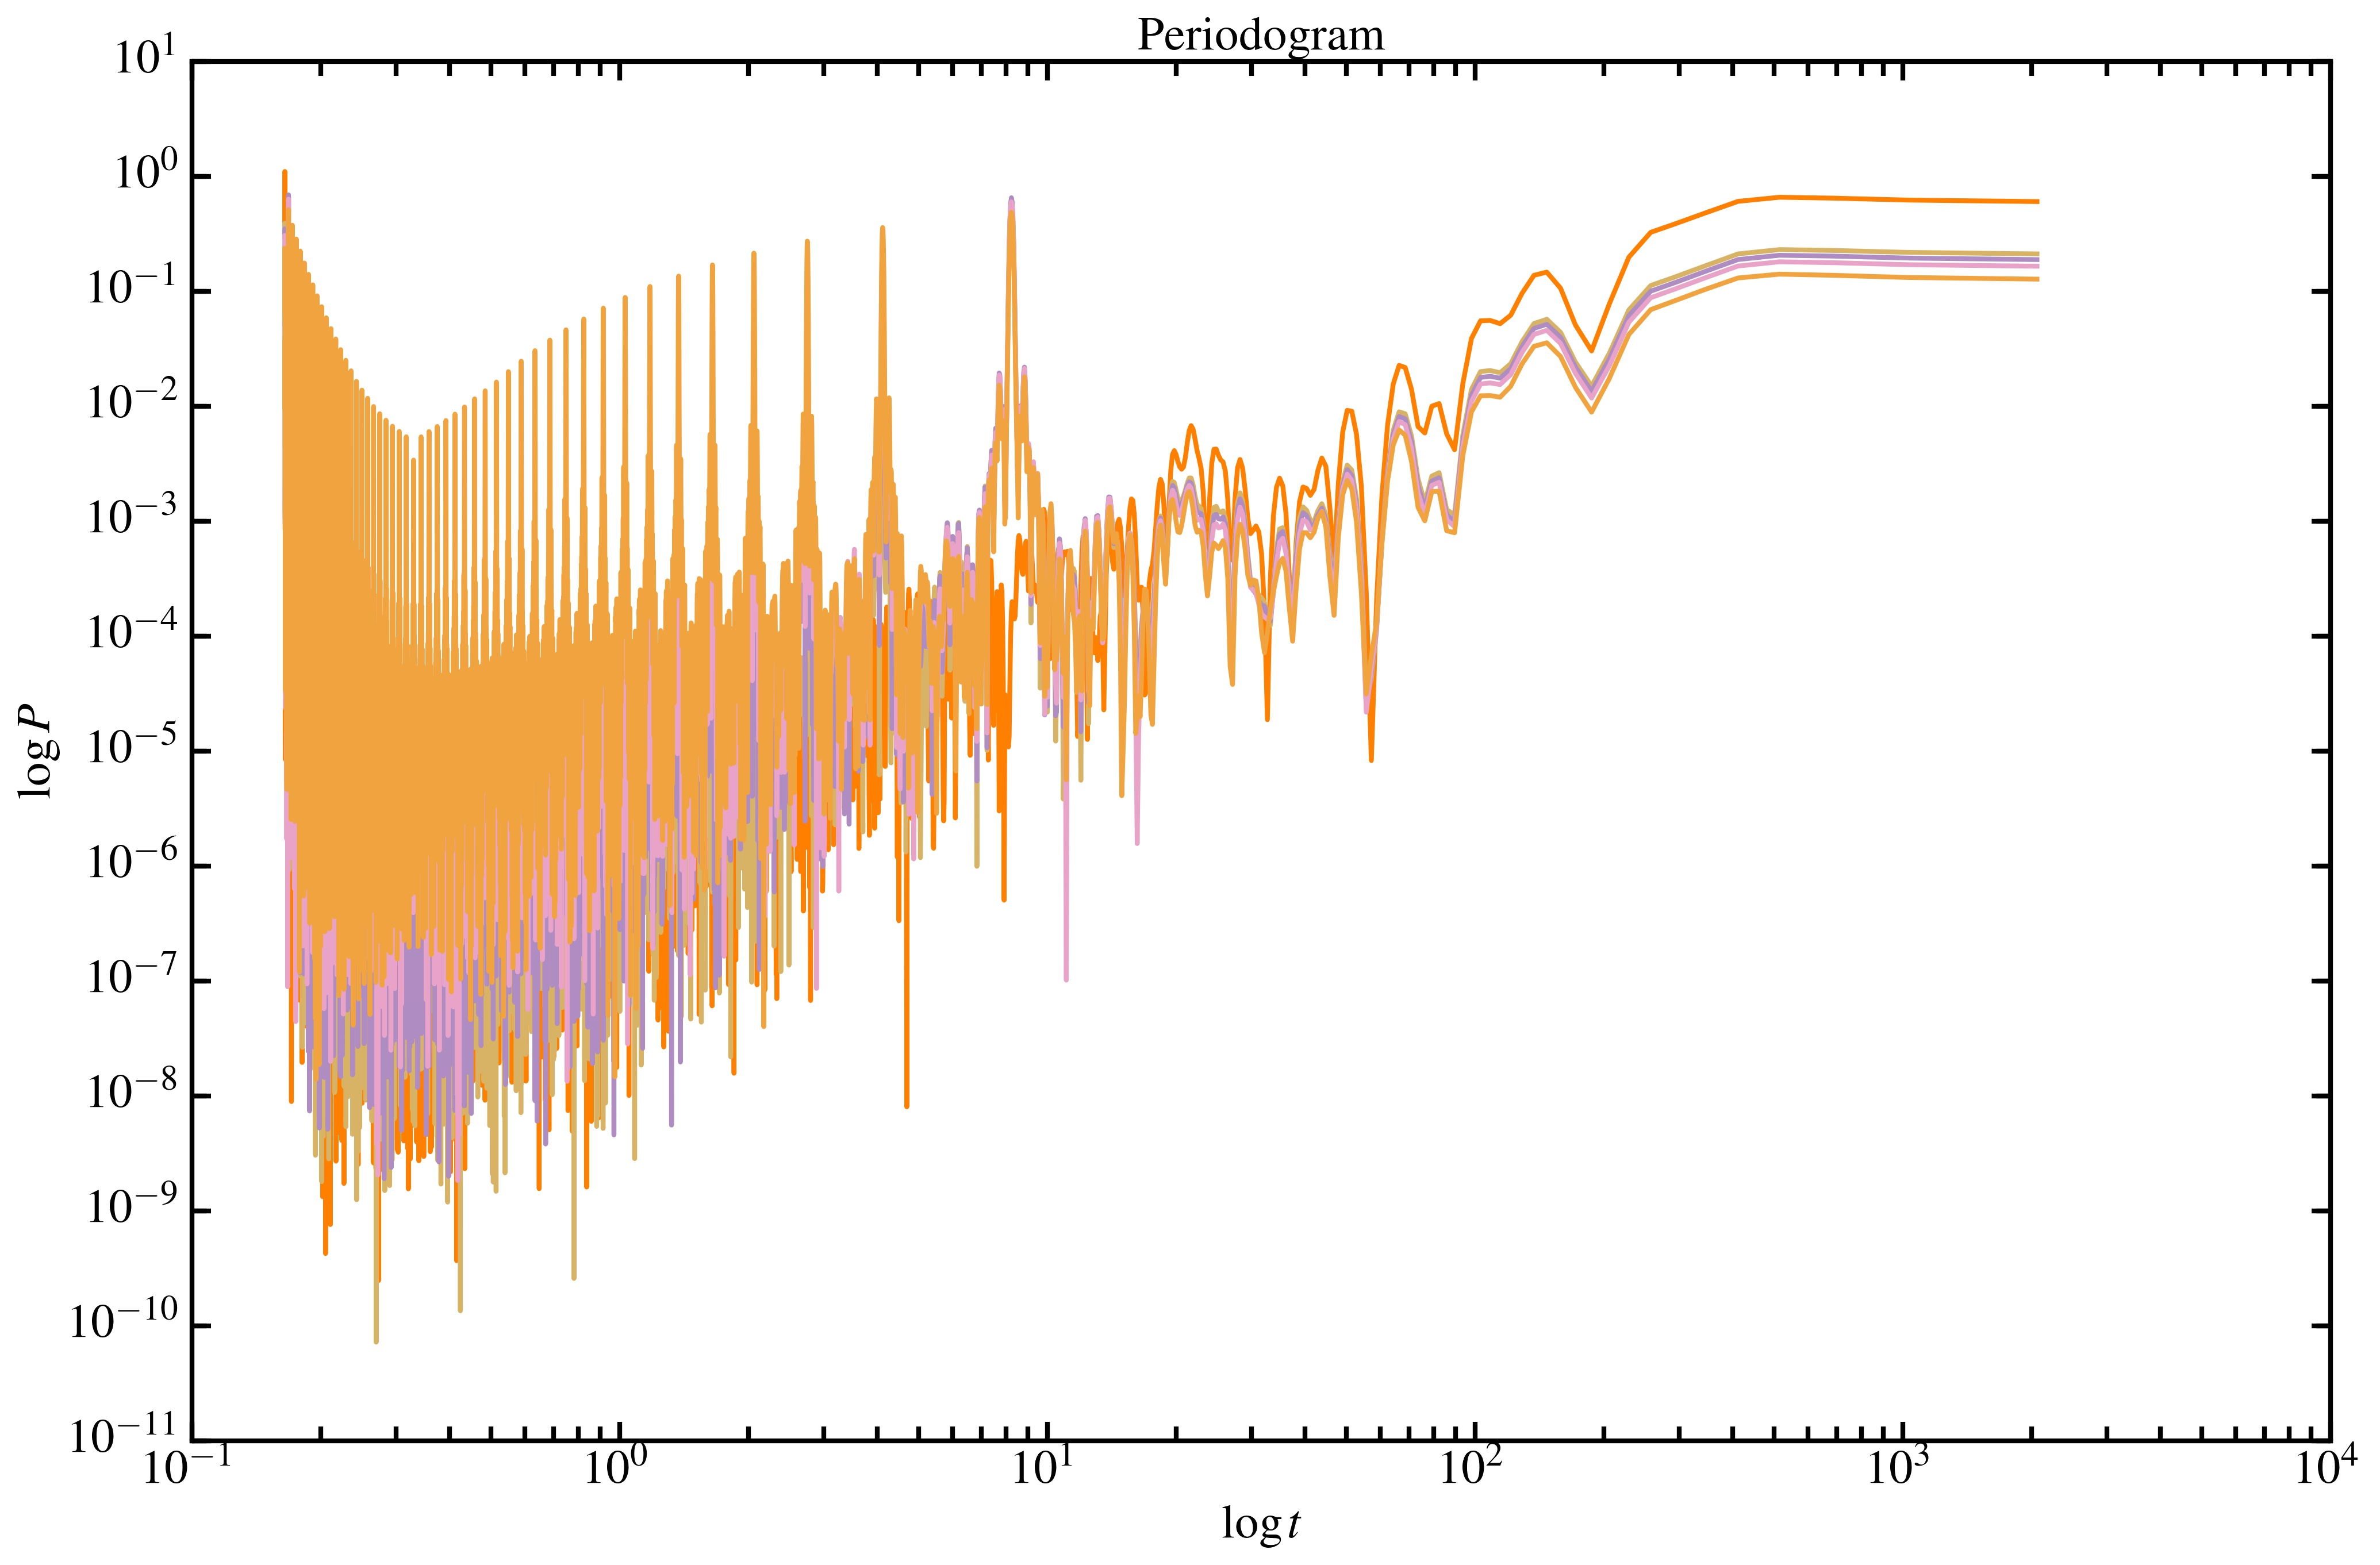
\includegraphics[scale=0.04]{images/Ps_full.jpg}
      \end{figure}
    \end{column}
    \begin{column}{0.5\textwidth}
        \begin{figure}
          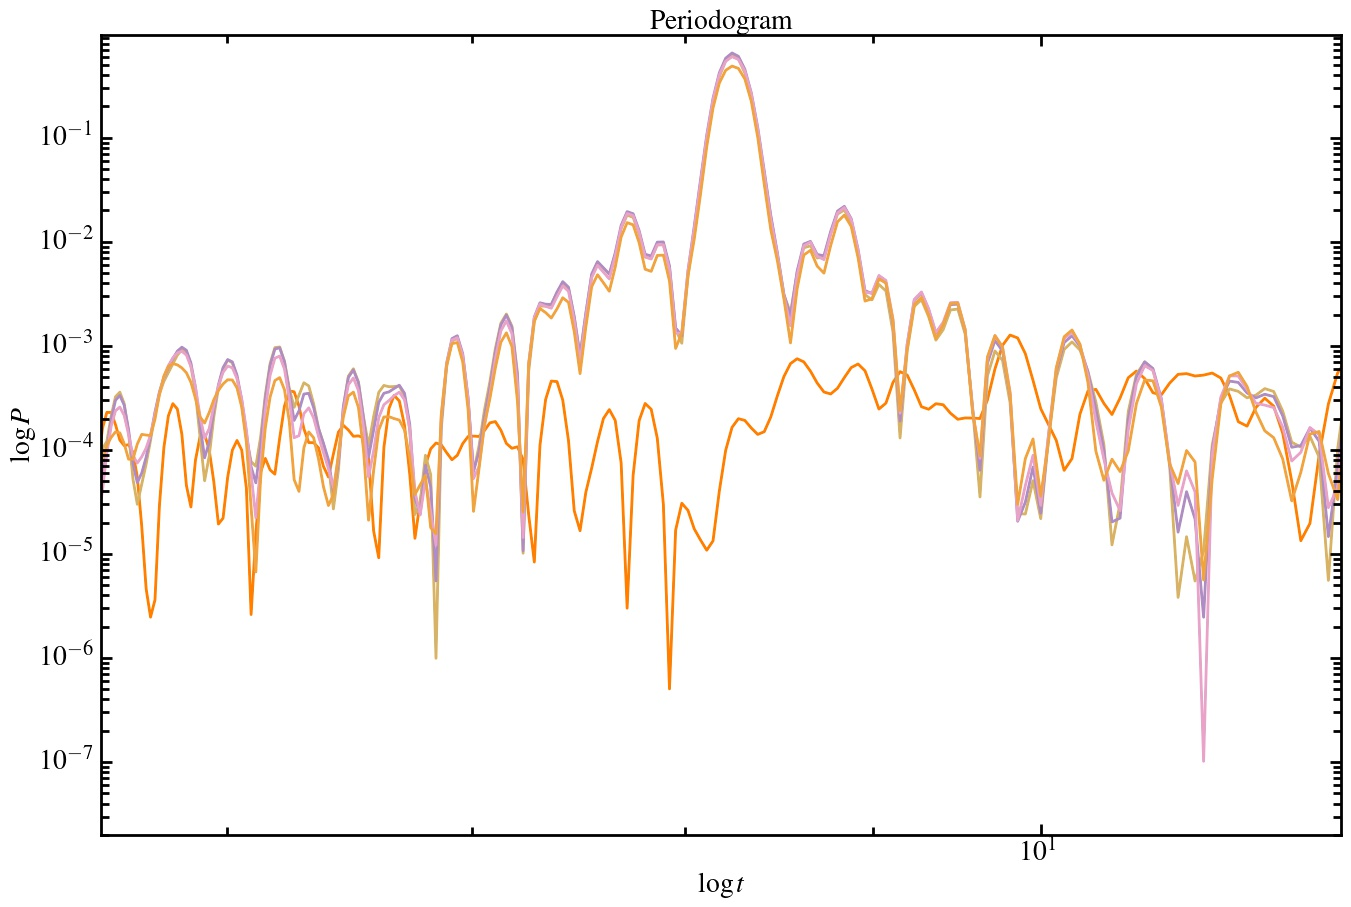
\includegraphics[scale=0.12]{images/Ps_detail.jpg}
        \end{figure}
    \end{column}
  \end{columns}
  \begin{columns}
  \centering
    \begin{column}{0.5\textwidth}
      \begin{itemize}
        \item $a_{1} = 10^{-4}$ pc
        \item $a_{2} = 10^{-4}$ pc
        \item $T = 8.25$ d
        \item $e$ ranges from 0.0 to 0.75
      \end{itemize}
    \end{column}
    \begin{column}{0.5\textwidth}
      \begin{itemize}
        \item $M_{12} = 138.68 \times 10^{6} M_{\odot}$
        \item $\Omega = 0.0$ degree
        \item $i = 90.0$ degree
      \end{itemize}
    \end{column}
  \end{columns}
\end{frame}

\begin{frame}
\frametitle{Massive Black Hole Binary Fit for PG 1302-102}
  \begin{figure}
    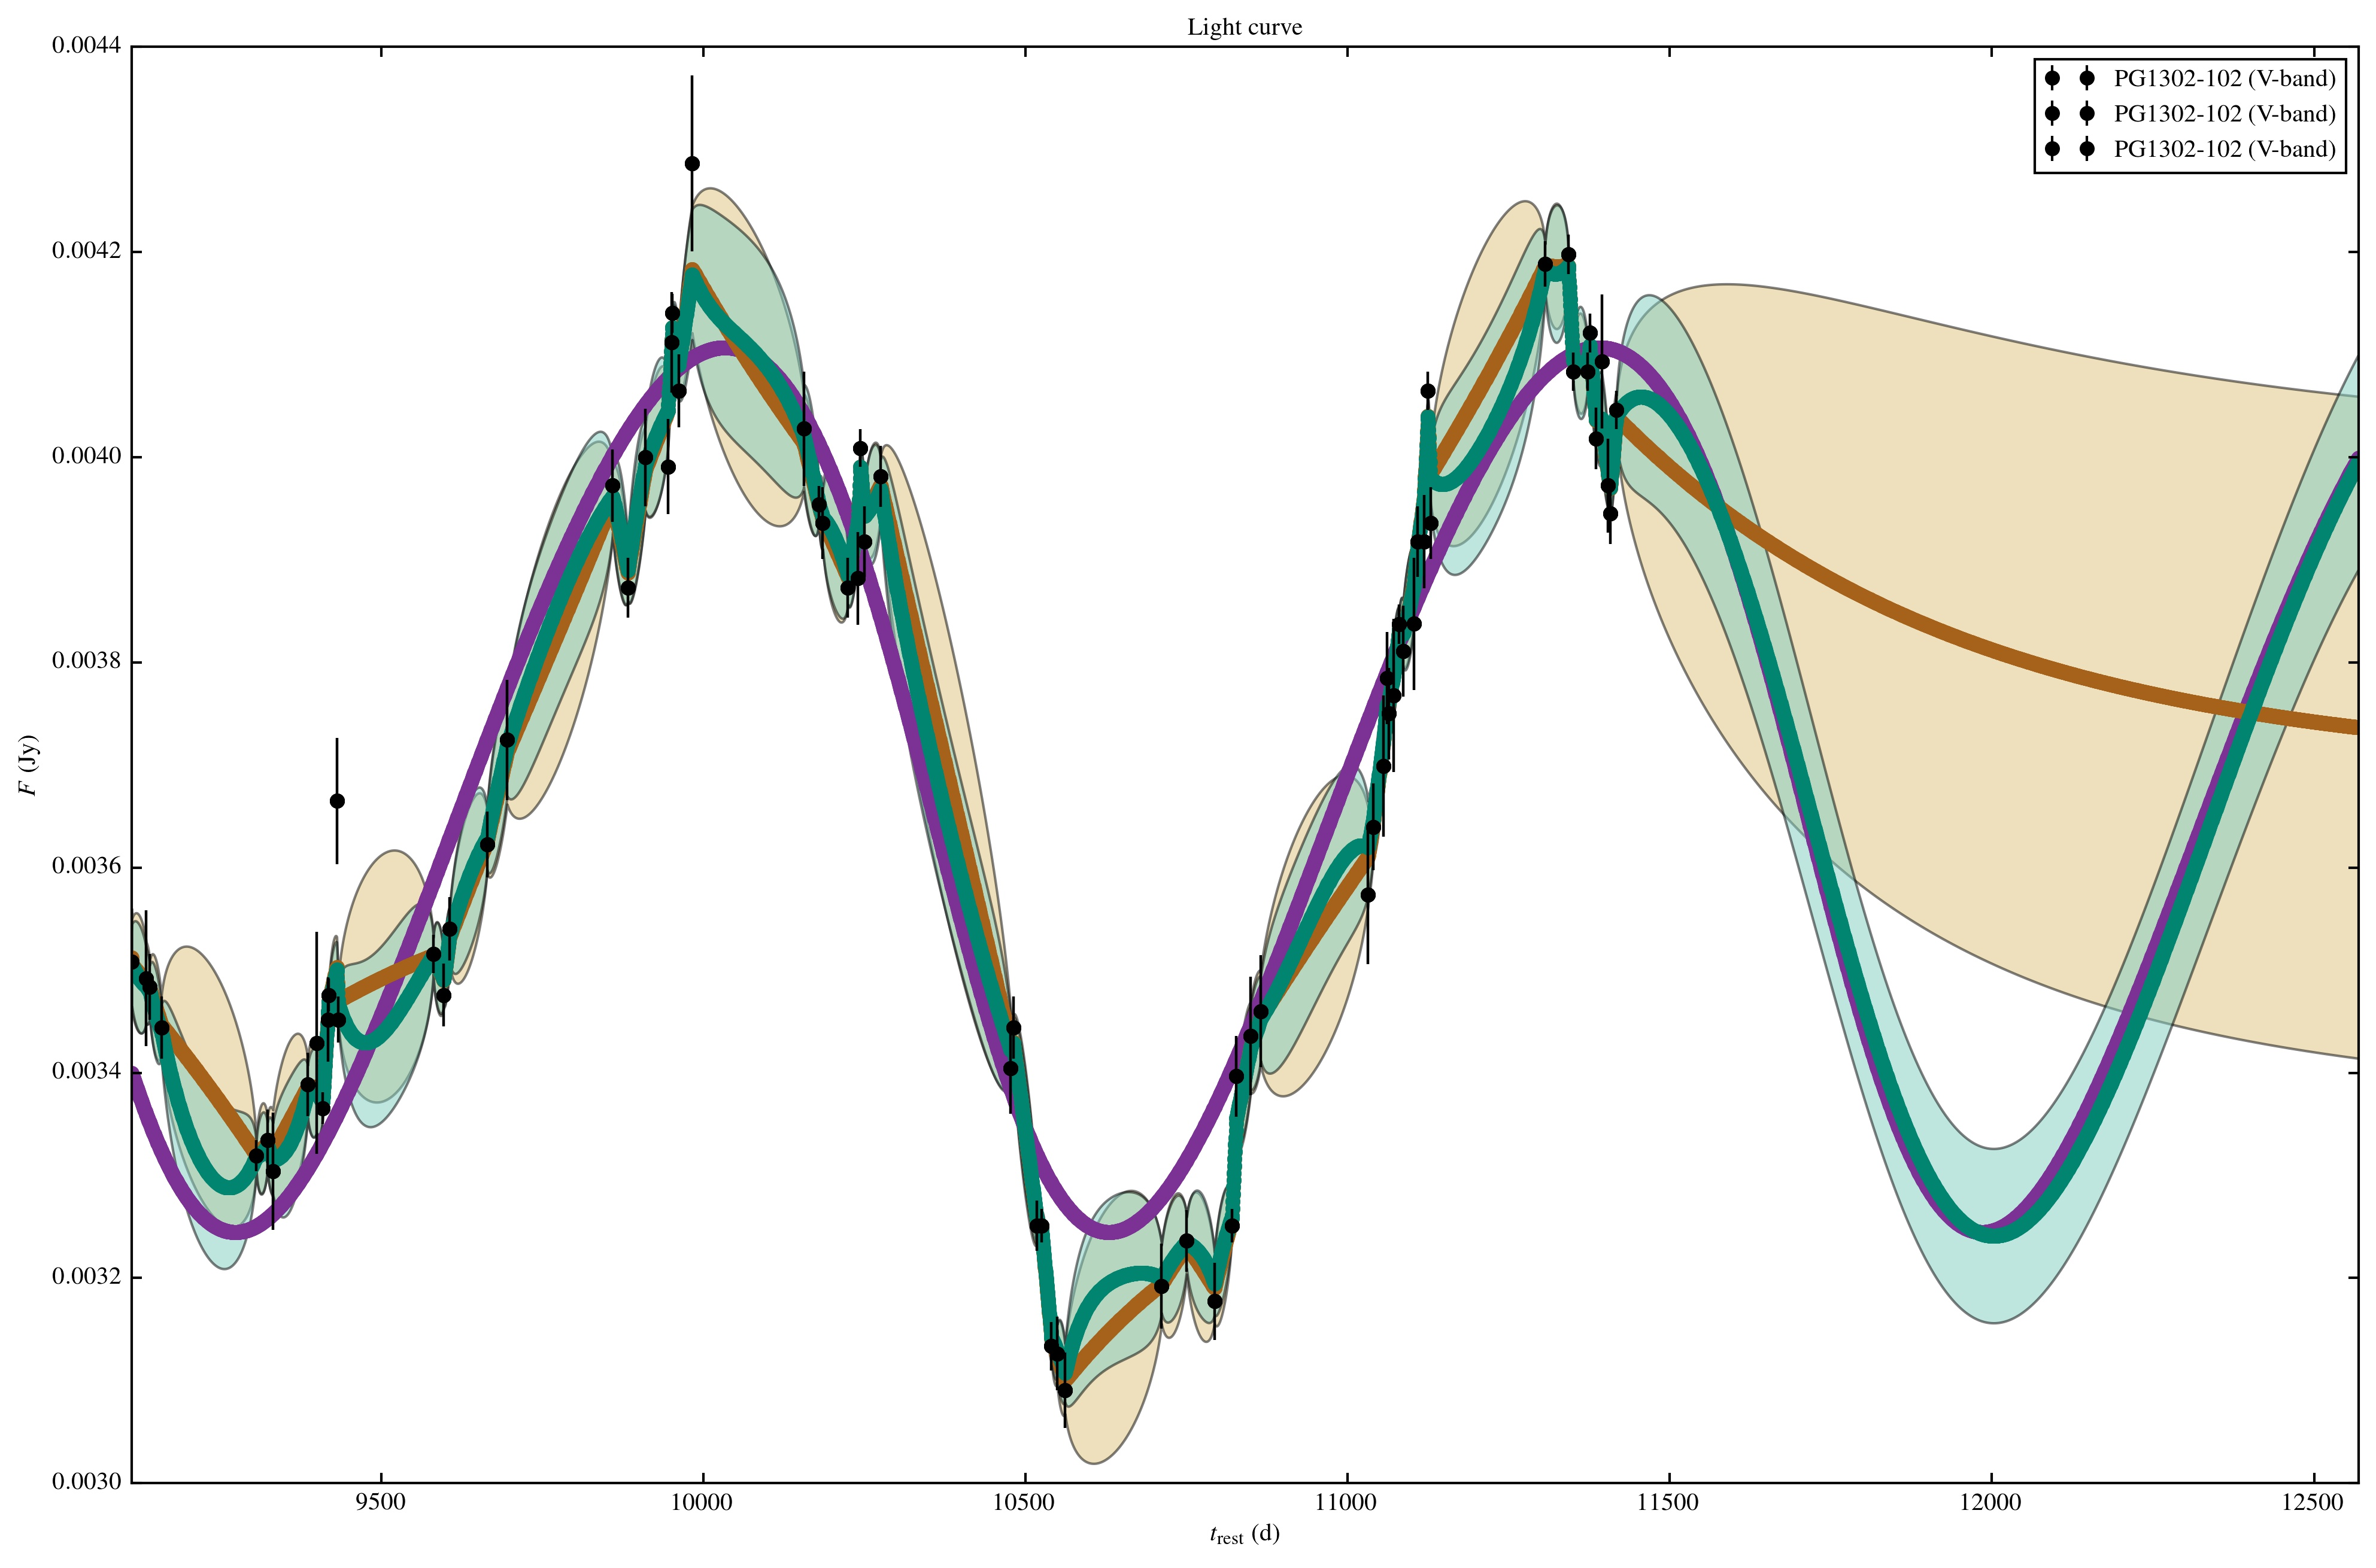
\includegraphics[scale=0.05]{images/PG1302-102_LC.jpg}
  \end{figure}
  \begin{columns}
  \centering
    \begin{column}{0.5\textwidth}
      \begin{itemize}
        \item {\scriptsize $a_{1} \sim 6.8 \times 10^{-3}$~pc}
        \item {\scriptsize $a_{2} \sim 1.1 \times 10^{-2}$~pc}
        \item {\scriptsize $T \sim 1343$~d}
      \end{itemize}
    \end{column}
    \begin{column}{0.5\textwidth}
      \begin{itemize}
        \item {\scriptsize $M_{12} \sim 4.05 \times 10^{9} M_{\odot}$}
        \item {\scriptsize $M_{2}/M_{1} \sim 0.66$}
        \item {\scriptsize $e \sim 0.077$}
      \end{itemize}
    \end{column}
  \end{columns}
\end{frame}

\appendix
\begin{frame}[allowframebreaks]
  \bibliography{../TeX/bibliography/allrefs}
\end{frame}

\end{document}
